% =====================================================================
% BMED365 (Spring 2027) — Lab 4: Differentiable Neurosymbolic AI Report
% Printable Companion Notebook Export: 01_data_geometry_and_prior_audit.ipynb
% Compile with: pdflatex 01_data_geometry_and_prior_audit_ipynb.tex (run twice)
% =====================================================================
\documentclass[10pt,a4paper]{article}

\usepackage[utf8]{inputenc}
\usepackage[T1]{fontenc}
\usepackage[english]{babel}
\usepackage{lmodern}
\usepackage{microtype}
\usepackage{graphicx}
\usepackage{booktabs}
\usepackage{xltabular}
\usepackage{tabularx}
\usepackage{array}
\usepackage[table]{xcolor}
\usepackage{amsmath,amssymb,mathtools}
\usepackage{enumitem}
\usepackage[margin=1.7cm,top=1.75cm,bottom=1.85cm,headheight=14pt]{geometry}
\usepackage{fancyhdr}
\usepackage{lastpage}
\usepackage{titlesec}
\usepackage[most]{tcolorbox}
\usepackage{listings}
\usepackage{float}
\usepackage{caption}
\usepackage[hyphens]{url}
\usepackage[
    colorlinks=true,
    linkcolor=uibblue,
    citecolor=uibblue,
    urlcolor=uibred,
    bookmarksnumbered=true,
    bookmarksopen=true,
    pdftitle={01_data_geometry_and_prior_audit.ipynb -- 7T MRI Geometry and Empirical Biophysical Prior Audit (BMED365 Spring 2027)},
    pdfauthor={Arvid Lundervold (University of Bergen & MMIV) -- BMED365 Spring 2027},
    pdfsubject={BMED365 Spring 2027 -- Differentiable Neurosymbolic AI Companion Notebook}
]{hyperref}
\def\UrlBreaks{\do\/\do-\do_\do.}
% Allow clean line breaks after underscores in long filenames & Python identifiers
\let\origunderscore\_
\renewcommand{\_}{\origunderscore\allowbreak}

% =====================================================================
% COLORS (UiB / MMIV / BMED365 House Style)
% =====================================================================
\definecolor{uibblue}{RGB}{0, 61, 115}
\definecolor{uibred}{RGB}{175, 28, 44}
\definecolor{kiwigreen}{RGB}{27, 138, 90}
\definecolor{amberwarn}{RGB}{165, 95, 0}
\definecolor{amberbg}{RGB}{255, 250, 240}
\definecolor{lightgray}{RGB}{246, 248, 250}
\definecolor{rowalt}{RGB}{243, 247, 252}
\definecolor{codebg}{RGB}{245, 248, 252}
\definecolor{codehdr}{RGB}{224, 234, 246}
\definecolor{outbg}{RGB}{250, 250, 250}
\definecolor{outhdr}{RGB}{236, 238, 240}
\definecolor{codekw}{RGB}{0, 75, 145}
\definecolor{codestr}{RGB}{155, 35, 45}
\definecolor{codecmt}{RGB}{90, 105, 118}

% =====================================================================
% TYPOGRAPHY, HEADERS & CALLOUT BOXES
% =====================================================================
\setlength{\parindent}{0pt}
\setlength{\parskip}{0.42em}
\setlength{\emergencystretch}{1.8em}
\setlist[itemize]{topsep=2pt,itemsep=2pt,leftmargin=1.45em}
\setlist[enumerate]{topsep=2pt,itemsep=2pt,leftmargin=1.65em}

\newcolumntype{L}[1]{>{\raggedright\arraybackslash}p{#1}}
\newcolumntype{C}[1]{>{\centering\arraybackslash}p{#1}}
\newcolumntype{R}[1]{>{\raggedleft\arraybackslash}p{#1}}
\newcolumntype{Y}{>{\raggedright\arraybackslash}X}

\titleformat{\section}{\large\bfseries\color{uibblue}}{\thesection}{0.65em}{}[\vspace{1pt}\color{uibblue!40}\titlerule]
\titleformat{\subsection}{\normalsize\bfseries\color{uibblue!88!black}}{\thesubsection}{0.55em}{}
\titleformat{\subsubsection}{\small\bfseries\color{uibblue!75!black}}{\thesubsubsection}{0.5em}{}
\titlespacing*{\section}{0pt}{1.05em}{0.4em}
\titlespacing*{\subsection}{0pt}{0.75em}{0.25em}
\titlespacing*{\subsubsection}{0pt}{0.55em}{0.2em}

\pagestyle{fancy}
\fancyhf{}
\fancyhead[L]{\footnotesize\textcolor{gray}{BMED365 (Spring 2027) $\cdot$ Neurosymbolic 7\,T MRI Package}}
\fancyhead[R]{\footnotesize\textcolor{gray}{\texttt{01\_data\_geometry\_and\_prior\_audit.ipynb}}}
\fancyfoot[L]{\footnotesize\textcolor{gray}{University of Bergen \& MMIV $\cdot$ \href{https://github.com/arvidl/BMED365-2027}{\textcolor{gray}{github.com/arvidl/BMED365-2027}}}}
\fancyfoot[R]{\footnotesize\textcolor{gray}{Page \thepage{} of \pageref{LastPage}}}
\renewcommand{\headrulewidth}{0.4pt}
\renewcommand{\footrulewidth}{0.2pt}

\fancypagestyle{firstpage}{
    \fancyhf{}
    \fancyfoot[L]{\footnotesize\textcolor{gray}{University of Bergen \& MMIV $\cdot$ \href{https://github.com/arvidl/BMED365-2027}{\textcolor{gray}{github.com/arvidl/BMED365-2027}}}}
    \fancyfoot[R]{\footnotesize\textcolor{gray}{Page \thepage{} of \pageref{LastPage}}}
    \renewcommand{\headrulewidth}{0pt}
    \renewcommand{\footrulewidth}{0.2pt}
}

% --- Notebook Cell & Pedagogical Boxes ---
\newtcolorbox{seqbox}[1][]{
    enhanced, breakable,
    colback=lightgray, colframe=uibblue,
    colbacktitle=uibblue, coltitle=white,
    fonttitle=\bfseries\small, title={#1},
    boxrule=0.6pt, arc=2.5pt, left=7pt, right=7pt, top=5pt, bottom=5pt
}

\newtcolorbox{codebox}[1][]{
    enhanced, breakable,
    colback=codebg, colframe=uibblue!35,
    colbacktitle=codehdr, coltitle=uibblue!90!black,
    fonttitle=\ttfamily\scriptsize\bfseries, title={#1},
    boxrule=0.55pt, arc=2.2pt, left=6pt, right=6pt, top=3pt, bottom=3pt,
    toptitle=2.5pt, bottomtitle=2.5pt
}

\newtcolorbox{outbox}[1][]{
    enhanced, breakable,
    colback=outbg, colframe=gray!45,
    colbacktitle=outhdr, coltitle=black!75,
    fonttitle=\ttfamily\scriptsize\bfseries, title={#1},
    boxrule=0.5pt, arc=2.2pt, left=6pt, right=6pt, top=3pt, bottom=3pt,
    toptitle=2pt, bottomtitle=2pt
}

\newtcolorbox{clinbox}[1][]{
    enhanced, breakable,
    colback=amberbg, colframe=amberwarn,
    colbacktitle=amberwarn, coltitle=white,
    fonttitle=\bfseries\small, title={#1},
    boxrule=0.6pt, arc=2.5pt, left=7pt, right=7pt, top=5pt, bottom=5pt
}

\newtcolorbox{guidehdr}[1][]{
    enhanced,
    colback=kiwigreen!6, colframe=kiwigreen!75!black,
    borderline west={2.5pt}{0pt}{kiwigreen!85!black},
    boxrule=0.45pt, arc=2pt, left=7pt, right=7pt, top=3.5pt, bottom=3.5pt,
    before skip=0.7em, after skip=0.35em
}

% --- Listings Styles (UTF-8 literate support for pdflatex) ---
\lstdefinestyle{pybmed}{
    language=Python,
    basicstyle=\ttfamily\scriptsize,
    keywordstyle=\bfseries\color{codekw},
    stringstyle=\color{codestr},
    commentstyle=\itshape\color{codecmt},
    showstringspaces=false,
    breaklines=true,
    breakatwhitespace=false,
    breakindent=12pt,
    columns=fullflexible,
    keepspaces=true,
    upquote=true,
    aboveskip=2pt,
    belowskip=2pt,
    xleftmargin=0pt,
    xrightmargin=0pt,
    literate={±}{{$\pm$}}1
             {³}{{\textsuperscript{3}}}1
             {×}{{$\times$}}1
             {é}{{\'e}}1
             {ö}{{\"o}}1
             {Ł}{{\L{}}}1
             {Δ}{{$\Delta$}}1
             {α}{{$\alpha$}}1
             {–}{{--}}1
             {—}{{---}}1
             {≥}{{$\ge$}}1
             {≤}{{$\le$}}1
             {⊂}{{$\subset$}}1
             {∈}{{$\in$}}1
             {→}{{$\to$}}1
             {…}{{\ldots}}1
}

\lstdefinestyle{bashbmed}{
    language=bash,
    basicstyle=\ttfamily\scriptsize,
    keywordstyle=\bfseries\color{codekw},
    stringstyle=\color{codestr},
    commentstyle=\itshape\color{codecmt},
    showstringspaces=false,
    breaklines=true,
    breakatwhitespace=false,
    breakindent=12pt,
    columns=fullflexible,
    keepspaces=true,
    upquote=true,
    aboveskip=2pt,
    belowskip=2pt,
    xleftmargin=0pt,
    xrightmargin=0pt
}

\lstdefinestyle{outbmed}{
    basicstyle=\ttfamily\scriptsize\color{black!85},
    showstringspaces=false,
    breaklines=true,
    breakatwhitespace=false,
    columns=fullflexible,
    keepspaces=true,
    upquote=true,
    aboveskip=1pt,
    belowskip=1pt,
    xleftmargin=0pt,
    xrightmargin=0pt
}

\lstdefinestyle{outbmedwide}{
    basicstyle=\ttfamily\fontsize{6.3pt}{7.6pt}\selectfont\color{black!85},
    showstringspaces=false,
    breaklines=true,
    breakatwhitespace=false,
    columns=fullflexible,
    keepspaces=true,
    upquote=true,
    aboveskip=1pt,
    belowskip=1pt,
    xleftmargin=0pt,
    xrightmargin=0pt
}

\newcommand{\ghblob}{https://github.com/arvidl/BMED365-2027/blob/main}
\newcommand{\colabbase}{https://colab.research.google.com/github/arvidl/BMED365-2027/blob/main}
\newcommand{\repodir}{Lab4-Comp-Imag/Kiwi-challenge/docs/neurosymbolic-report}
\newcommand{\colabbtn}[1]{%
  \href{#1}{\tcbox[on line, arc=2.5pt, boxsep=0pt, left=6pt, right=6pt, top=2.5pt, bottom=2.5pt,
    colback=amberwarn!85!yellow, colframe=white!70!amberwarn, boxrule=0.5pt]{%
    \sffamily\bfseries\scriptsize\color{white}Open in Google Colab}}%
}

% =====================================================================
\begin{document}
\thispagestyle{firstpage}

% --- TITLE BANNER ---
\begin{tcolorbox}[
    enhanced, colback=uibblue, colframe=uibblue,
    arc=3.5pt, left=12pt, right=12pt, top=9pt, bottom=9pt
]
{\Large\bfseries\color{white} Companion Notebook 01 --- 7\,T MRI Geometry \& Empirical Biophysical Prior Audit\\[2pt]
{\large Verifying Botanical Placentation, 7\,T $T_2$ Core-vs.-Rim Physics, Steric Packing \& Micro-GT Provenance}}\\[4pt]
{\normalsize\color{white!90} BMED365 --- Computational Imaging, Modeling and AI in Biomedicine (Spring 2027)}\\[3pt]
{\footnotesize\color{white!84}
Arvid Lundervold (University of Bergen \& MMIV) $\;\cdot\;$ Reproduces Report Sec.\ 2.1--2.2, 3.1, Figs.\ 1--3 \& Table~3 $\;\cdot\;$ Measured runtime: \texttt{27.4 s} (MPS)
}\\[6pt]
\colabbtn{\colabbase/\repodir/notebooks/01_data_geometry_and_prior_audit.ipynb}\hspace{8pt}
{\footnotesize\href{\ghblob/\repodir/notebooks/01_data_geometry_and_prior_audit.ipynb}{\textcolor{white}{\underline{\texttt{01\_data\_geometry\_and\_prior\_audit.ipynb} on GitHub}}}}\hspace{10pt}
{\footnotesize\href{\ghblob/\repodir/neurosymbolic-kiwi-report.pdf}{\textcolor{white}{\underline{Technical Report PDF}}}}
\end{tcolorbox}

\begin{seqbox}[Neurosymbolic 7\,T MRI Technical Report --- Companion Package (\texttt{docs/neurosymbolic-report})]
{\footnotesize Companion to \href{\ghblob/\repodir/neurosymbolic-kiwi-report.pdf}{\textbf{\texttt{neurosymbolic-kiwi-report.pdf}}} and shared library \href{\ghblob/\repodir/notebooks/kiwi_ns_lib.py}{\texttt{kiwi\_ns\_lib.py}} (\href{\ghblob/\repodir/notebooks/kiwi_ns_lib_py.pdf}{\textit{annotated PDF}}):}
\begin{enumerate}[start=1, itemsep=1.2pt, topsep=2pt, font=\footnotesize]
    \item \textbf{\texttt{01\_data\_geometry\_and\_prior\_audit.ipynb} (this notebook)} --- 7\,T MRI geometry, empirical audit of Priors 1--3, tri-planar Micro-GT superimposition \& manual GT editing guide (Figs.\ 1--3, Table~3; 27.4\,s MPS).
    \item \href{\ghblob/\repodir/notebooks/02_instancenorm_trap_and_ltn_math.ipynb}{\texttt{02\_instancenorm\_trap\_and\_ltn\_math.ipynb}} --- Experimental proof of \texttt{InstanceNorm3d} coordinate erasure, Bayes Log-Odds \texttt{Organ-GPS}, fuzzy $T$-norms \& LTN $p$-mean autograd sweep (Figs.\ 4--5, Table~4; 7.2\,s MPS).
    \item \href{\ghblob/\repodir/notebooks/03_multiseed_ablation_and_calibration.ipynb}{\texttt{03\_multiseed\_ablation\_and\_calibration.ipynb}} --- 3-seed $\times$ 6-model controlled ablation, operating-point calibration shift \& unmasked whole-organ OOD safety (Figs.\ 6--7, Tables~5--6; 555.1\,s MPS).
    \item \href{\ghblob/\repodir/notebooks/04_mechanistic_interpretability_and_biomarkers.ipynb}{\texttt{04\_mechanistic\_interpretability\_and\_biomarkers.ipynb}} --- Causal neural--symbolic division of labor ($z_{\text{GPS}}$), Mat\'ern hard-core split sweep, error anatomy \& 128-slice NIfTI biomarkers (Figs.\ 8--9, Tables~7--8; 99.3\,s MPS).
    \item \href{\ghblob/\repodir/notebooks/05_axiom_stress_tests_and_clinical_translation.ipynb}{\texttt{05\_axiom\_stress\_tests\_and\_clinical\_translation.ipynb}} --- Pathological mass-effect center-shift ($\Delta r \in [0, 8]$\,mm) \& radial-scale ($\alpha \in [0.80, 1.25]$) stress tests vs.\ rigid post-hoc masks (Fig.\ 10, Table~9; 55.4\,s MPS).
\end{enumerate}
\end{seqbox}

\subsection*{Purpose}
Before encoding any biological, physical, or geometric law into a differentiable neural loss, we must \textbf{verify empirically} whether real ground-truth structures actually satisfy our priors. Here we:
\begin{enumerate}
\item Load the intact 2005 UiB 7\,T Bruker Pharmascan RARE kiwifruit MRI (\texttt{256 $\times$ 256 $\times$ 128}, anisotropic voxel spacing \texttt{0.2344 $\times$ 0.2344 $\times$ 0.5000 mm\textsuperscript{3}}) and curated 3D Micro-Ground-Truth (\texttt{98} 3D seed instances).
\item Construct the intrinsic normalized organ coordinate frame $(r/R_{\text{fruit}}(z),\, |2z/Z - 1|)$ and smooth differentiable predicates $R_{\text{ring}}(\mathbf{x})$ (botanical axile placentation) and $B_{\text{non-dark}}(\mathbf{x})$ (7\,T Bloch $T_2$ contrast at \texttt{TE = 63.9 ms}).
\item Audit \textbf{core vs. 1-voxel partial-volume rim} contrast physics and measure the empirical 3D single-seed volume and nearest-neighbor steric spacing distribution (\texttt{Lab 5} Mat\'ern hard-core prior).
\end{enumerate}

\section*{0. Environment Setup: Portable Execution, Shared Library \& 3D Imaging Stack}
\addcontentsline{toc}{section}{\texorpdfstring{0. Environment Setup: Portable Execution, Shared Library \& 3D Imaging Stack}{0. Environment Setup: Portable Execution, Shared Library and 3D Imaging Stack}}

\begin{guidehdr}
{\small\bfseries\color{kiwigreen!75!black}Conceptual \& Practical Motivation}
\end{guidehdr}
Before auditing any biophysical prior, we initialize a self-contained runtime that reproduces the exact same numbers locally (macOS Apple Silicon or Linux/\allowbreak{}CUDA) and in \textbf{Google Colab}:

\begin{itemize}
\item \textbf{Zero-drift shared library (\texttt{kiwi\_ns\_lib.py}):} All five companion notebooks import the exact same coordinate transforms, morphological operators, and metric evaluators from \texttt{kiwi\_ns\_lib.py} (automatically downloaded from GitHub \texttt{main} if opened standalone in Colab), eliminating code drift between notebooks and technical report equations.
\item \textbf{3D medical imaging \& geometry stack:}
\begin{itemize}
\item \texttt{nibabel} reads NIfTI-1 (\texttt{.nii.gz}) volumes together with their $4 \times 4$ physical affine header $\mathbf{A}$ (voxel spacing $s = (0.2344,\, 0.2344,\, 0.5000)\,\text{mm}$).
\item \texttt{scipy.ndimage} (\texttt{ndi}) performs 3D mathematical morphology (grayscale closing for $B_1$ shading removal and 1-voxel binary dilation to isolate partial-volume seed rims), while \texttt{scipy.spatial.distance.cdist} computes all pairwise physical 3D inter-seed distances in millimeters.
\item \texttt{skimage.measure.regionprops} extracts exact per-instance 3D voxel counts and centroids across all \texttt{98} curated seed IDs.
\item \texttt{torch}, \texttt{numpy}, \texttt{pandas}, and \texttt{matplotlib} support tensor utilities, summary tables (\textbf{Table 1}), and publication-quality figures (\textbf{Figures 1, 1b \& 2}).
\end{itemize}
\item \textbf{Runtime device \& output resolution:} \texttt{kns.get\_best\_device()} selects the fastest available backend (\texttt{CUDA} $\to$ Apple \texttt{MPS} $\to$ \texttt{CPU}), and \texttt{kns.resolve\_report\_dirs()} resolves \texttt{FIG\_DIR} and \texttt{RES\_DIR} for saving report figures and \texttt{nb01\_prior\_audit.json}.
\end{itemize}

\begin{codebox}[{In [1] $\cdot$ Python --- Environment setup, \texttt{kiwi\_ns\_lib.py} bootstrap \& output paths}]
\begin{lstlisting}[style=pybmed]
import json
import sys
import urllib.request
from pathlib import Path

# Auto-fetch shared library `kiwi_ns_lib.py` if opened standalone in Google Colab
if not Path("kiwi_ns_lib.py").exists():
    for cand in [Path("docs/neurosymbolic-report/notebooks/kiwi_ns_lib.py"),
                 Path("Lab4-Comp-Imag/Kiwi-challenge/docs/neurosymbolic-report/notebooks/kiwi_ns_lib.py")]:
        if cand.exists():
            sys.path.insert(0, str(cand.parent.resolve()))
            break
    else:
        url = "https://raw.githubusercontent.com/arvidl/BMED365-2027/main/Lab4-Comp-Imag/Kiwi-challenge/docs/neurosymbolic-report/notebooks/kiwi_ns_lib.py"
        print("Downloading kiwi_ns_lib.py from GitHub main for Colab session...")
        urllib.request.urlretrieve(url, "kiwi_ns_lib.py")

if str(Path.cwd()) not in sys.path:
    sys.path.insert(0, str(Path.cwd()))

import importlib.util
for pkg in ("nibabel", "torch"):
    if importlib.util.find_spec(pkg) is None:
        import subprocess
        subprocess.check_call([sys.executable, "-m", "pip", "install", "-q", pkg])

get_ipython().run_line_magic("matplotlib", "inline")
import matplotlib.pyplot as plt
import numpy as np
import pandas as pd
import torch
from scipy import ndimage as ndi
from scipy.spatial.distance import cdist
from skimage import measure

plt.rcParams.update({"figure.dpi": 130, "savefig.dpi": 200, "font.size": 9.5})

import kiwi_ns_lib as kns

DEVICE = kns.get_best_device()
FIG_DIR, RES_DIR = kns.resolve_report_dirs()
print(f"Device: {DEVICE} | Figures -> {FIG_DIR} | Results -> {RES_DIR}")
\end{lstlisting}
\end{codebox}
\begin{outbox}[{Out [1] $\cdot$ stdout}]
\begin{lstlisting}[style=outbmed]
Device: mps | Figures -> <BMED365-2027>/Lab4-Comp-Imag/Kiwi-challenge/docs/neurosymbolic-report/figures | Results -> <BMED365-2027>/Lab4-Comp-Imag/Kiwi-challenge/docs/neurosymbolic-report/results
\end{lstlisting}
\end{outbox}

\section*{1. Load 7\,T MRI, Construct Organ Coordinates \& Audit All Three Priors}
\addcontentsline{toc}{section}{\texorpdfstring{1. Load 7\,T MRI, Construct Organ Coordinates \& Audit All Three Priors}{1. Load 7T MRI, Construct Organ Coordinates and Audit All Three Priors}}

Every biophysical parameter is verified quantitatively on the \texttt{98} curated 3D Micro-GT seeds before a single neural weight is trained.

\begin{guidehdr}
{\small\bfseries\color{kiwigreen!75!black}Conceptual \& Mathematical Guide: Formulating \& Empirically Auditing Three Biophysical Priors}
\end{guidehdr}

\subsubsection*{1.1 Scientific Principle \& Extreme Label Scarcity}
A core rule of trustworthy neurosymbolic biomedical AI is that \textbf{every symbolic prior must be tested as a falsifiable empirical hypothesis before it is compiled into a neural loss}. Inside the intact $256 \times 256 \times 128$ 7\,T RARE kiwifruit MRI, each anisotropic voxel is a rectangular brick of dimensions $s = (0.2344,\, 0.2344,\, 0.5000)\,\text{mm}$ and physical volume $v_{\text{vox}} = s_x s_y s_z = 0.02747\,\text{mm}^3$. Summing over the intact berry mask $M_{\text{fruit}}$ yields $V_{\text{kiwi}} = |M_{\text{fruit}}| \cdot v_{\text{vox}} / 1000 \approx 85.97\,\text{cm}^3$, of which the \texttt{59} labeled training seeds occupy only \textbf{$0.083\%$} of berry voxels---making verified domain laws essential to constrain the remaining $99.9\%$ of the organ.

\subsubsection*{1.2 Mathematical Definitions of Priors 1--3 (\texttt{kns.load\_kiwi\_dataset()})}
\begin{enumerate}
\item \textbf{Prior 1 --- Botanical Axile Placentation (\texttt{r\_norm}, \texttt{soft\_ring}):} On each axial slice $z$ with $\ge 80$ berry voxels, we compute the slice centroid $(c_x(z), c_y(z))$ and area-equivalent radius $R_{\text{fruit}}(z) = \sqrt{\text{Area}(z) / \pi}$, giving the dimensionless radial coordinate
\[
\tilde{r}(\mathbf{x}) = \operatorname{clip}\!\left(\frac{\sqrt{(x - c_x(z))^2 + (y - c_y(z))^2}}{R_{\text{fruit}}(z)},\, 0,\, 1.5\right).
\]
Botanical anatomy confines seeds to the inner-pericarp ring $\tilde{r} \in [0.22, 0.65]$ and non-polar slices $z \in [16, 111]$, encoded as a smooth differentiable membership field $R_{\text{ring}}(\mathbf{x}) \in [0, 1]$:
\[
R_{\text{ring}}(\mathbf{x}) = \sigma\!\left(\frac{\tilde{r}(\mathbf{x}) - 0.22}{0.02}\right)\sigma\!\left(\frac{0.65 - \tilde{r}(\mathbf{x})}{0.02}\right) g_z(z)\, M_{\text{fruit}}(\mathbf{x}),
\]
with 5-slice linear polar ramps $g_z(z) = \operatorname{clip}\!\left(\frac{z - 16}{5},\, 0,\, 1\right)\operatorname{clip}\!\left(\frac{111 - z}{5},\, 0,\, 1\right)$.
\item \textbf{Prior 2 --- $B_1$-Invariant 7\,T $T_2$ Contrast \& Partial-Volume Physics (\texttt{t2\_ratio}, \texttt{non\_dark}):} At 7\,T spin-echo RARE ($\text{TE} = 63.9\,\text{ms}$, $\text{TR} = 18{,}520.8\,\text{ms}$), signal decays as $S(\mathbf{x}) \propto \rho(\mathbf{x})(1 - e^{-\text{TR}/T_1})e^{-\text{TE}/T_2}$, rendering hydrated mucilage gel bright ($T_2 \sim 80$--$150\,\text{ms}$) and lignified seed coats deeply hypointense ($T_2 \sim 5$--$15\,\text{ms}$). Because ultra-high-field RF inhomogeneity adds centimeter-scale multiplicative shading $I_{\text{obs}}(\mathbf{x}) = B_1(\mathbf{x})S(\mathbf{x}) + \varepsilon(\mathbf{x})$, we estimate the local bright-gel envelope $E_{\text{local}}(\mathbf{x})$ via 3D grayscale morphological closing ($7 \times 7 \times 3$ structuring element) so dividing cancels $B_1$ locally:
\[
r_{T_2}(\mathbf{x}) = \operatorname{clip}\!\left(\frac{I(\mathbf{x})}{E_{\text{local}}(\mathbf{x}) + 0.03},\, 0,\, 1.25\right) \approx \frac{S(\mathbf{x})}{S_{\text{mucilage}}(\mathbf{x})}.
\]
The smooth physics penalty flags voxels that are either bright relative to local gel ($r_{T_2} > 0.82$) \textit{or} embedded in dry/\allowbreak{}air tissue lacking hydrated mucilage ($E_{\text{local}} < 0.32$):
\[
B_{\text{non\_dark}}(\mathbf{x}) = \max\!\left(\operatorname{clip}\!\left(\frac{r_{T_2}(\mathbf{x}) - 0.82}{0.15},\, 0,\, 1\right),\; \operatorname{clip}\!\left(\frac{0.32 - E_{\text{local}}(\mathbf{x})}{0.10},\, 0,\, 1\right)\right).
\]
\textbf{Why we explicitly audit \texttt{seed\_core} vs. 1-voxel \texttt{seed\_rim}:} Because $\Delta z = 0.50\,\text{mm}$ is $2.13\times$ thicker than in-plane spacing, boundary voxels mix dark seed ($r_{T_2} \approx 0.12$) and bright gel ($r_{T_2} \approx 0.90$) by partial-volume averaging $I_{\text{PV}} = \alpha I_{\text{seed}} + (1 - \alpha) I_{\text{gel}}$ (yielding $\approx 0.51$ for a 50/\allowbreak{}50 voxel). Dilating the GT mask by 1 voxel (\texttt{seed\_rim = binary\_dilation(seed\_core) \& \textasciitilde{}seed\_core}) verifies that placing the ramp onset at $0.82$ protects $100\%$ of seed cores and $>93\%$ of partial-volume rims from boundary erosion!
\item \textbf{Prior 3 --- Mat\'ern Steric Hard-Core Packing (\texttt{gt\_vols\_mm3}, \texttt{gt\_nn\_mm}):} Solid biological seeds cannot interpenetrate; their physical millimeter centroids must satisfy a hard-core floor $\|\mathbf{c}_i - \mathbf{c}_j\|_2 \ge d_{\min} = 0.88\,\text{mm}$, with single-seed volume well below the clump-splitting cutoff $V_{\text{split}} = 2.55\,\text{mm}^3$.
\end{enumerate}

\subsubsection*{1.3 What the Code Below Computes (Table 1)}
Loads the 7\,T MRI and Micro-GT, computes per-seed 3D volumes and pairwise physical nearest-neighbor distances (\texttt{cdist}), compares \texttt{t2\_ratio} and \texttt{non\_dark} across \texttt{seed\_core}, \texttt{seed\_rim}, and \texttt{non\_seed\_gel}, saves all \texttt{25} metrics to \texttt{../\allowbreak{}results/\allowbreak{}nb01\_prior\_audit.json}, and displays the summary table.

\begin{codebox}[{In [2] $\cdot$ Python --- Load 7\,T MRI, compute 3D physical seed stats \& audit Priors 1--3}]
\begin{lstlisting}[style=pybmed]
ds = kns.load_kiwi_dataset()

n_roi = len(np.unique(ds.roi_gt)) - 1
n_train = len(np.unique(ds.train_gt)) - 1
n_test = len(np.unique(ds.test_gt)) - 1
v_kiwi_cm3 = float(ds.fruit_mask.sum()) * ds.vox_vol_mm3 / 1000.0
labeled_frac_pct = 100.0 * float((ds.train_gt > 0).sum()) / float(ds.fruit_mask.sum())

# Measure 3D physical properties of all 98 curated Micro-GT seed instances
gt_props = measure.regionprops(ds.roi_gt)
gt_vols_mm3 = np.array([p.area * ds.vox_vol_mm3 for p in gt_props], dtype=np.float32)
gt_centroids_mm = np.array([
    [(p.centroid[0] + ds.rx0) * ds.spacing[0],
     (p.centroid[1] + ds.ry0) * ds.spacing[1],
     (p.centroid[2] + ds.rz0) * ds.spacing[2]]
    for p in gt_props
], dtype=np.float32)
dmat = cdist(gt_centroids_mm, gt_centroids_mm)
np.fill_diagonal(dmat, np.inf)
gt_nn_mm = dmat.min(axis=1)

# Voxel-level prior verification: GT seed cores vs 1-voxel partial-volume rims vs surrounding gel/tissue
roi_r = ds.r_norm[ds.rx0:ds.rx1, ds.ry0:ds.ry1, ds.rz0:ds.rz1]
roi_ring = ds.soft_ring[ds.rx0:ds.rx1, ds.ry0:ds.ry1, ds.rz0:ds.rz1]
roi_t2r = ds.t2_ratio[ds.rx0:ds.rx1, ds.ry0:ds.ry1, ds.rz0:ds.rz1]
roi_nd = ds.non_dark[ds.rx0:ds.rx1, ds.ry0:ds.ry1, ds.rz0:ds.rz1]
roi_fg = ds.fruit_mask[ds.rx0:ds.rx1, ds.ry0:ds.ry1, ds.rz0:ds.rz1]

seed_core = ds.roi_gt > 0
seed_rim = ndi.binary_dilation(seed_core, iterations=1) & (~seed_core)
non_seed_gel = roi_fg & (~seed_core) & (~seed_rim) & (roi_ring >= 0.5)

gt_r_cent = np.array([
    roi_r[int(round(p.centroid[0])), int(round(p.centroid[1])), int(round(p.centroid[2]))]
    for p in gt_props
], dtype=np.float32)

audit = {
    "volume_shape": list(ds.vol.shape),
    "spacing_mm": [round(s, 4) for s in ds.spacing],
    "vox_vol_mm3": round(ds.vox_vol_mm3, 5),
    "v_kiwi_cm3": round(v_kiwi_cm3, 2),
    "n_roi_seeds": int(n_roi),
    "n_train_seeds": int(n_train),
    "n_test_seeds": int(n_test),
    "labeled_train_seed_vox_pct": round(labeled_frac_pct, 3),
    "prior1_pct_core_in_ring": round(100.0 * float((roi_ring[seed_core] >= 0.5).mean()), 2),
    "prior1_centroid_r_min": round(float(gt_r_cent.min()), 3),
    "prior1_centroid_r_max": round(float(gt_r_cent.max()), 3),
    "prior1_centroid_r_median": round(float(np.median(gt_r_cent)), 3),
    "prior2_core_t2r_median": round(float(np.median(roi_t2r[seed_core])), 3),
    "prior2_core_t2r_p99": round(float(np.percentile(roi_t2r[seed_core], 99)), 3),
    "prior2_core_pct_safe": round(100.0 * float((roi_nd[seed_core] <= 0.2).mean()), 2),
    "prior2_rim_t2r_median": round(float(np.median(roi_t2r[seed_rim])), 3),
    "prior2_rim_t2r_p75": round(float(np.percentile(roi_t2r[seed_rim], 75)), 3),
    "prior2_rim_pct_penalized": round(100.0 * float((roi_nd[seed_rim] > 0.2).mean()), 2),
    "prior2_gel_t2r_median": round(float(np.median(roi_t2r[non_seed_gel])), 3),
    "prior3_vol_median_mm3": round(float(np.median(gt_vols_mm3)), 2),
    "prior3_vol_iqr_mm3": [round(float(np.percentile(gt_vols_mm3, 25)), 2), round(float(np.percentile(gt_vols_mm3, 75)), 2)],
    "prior3_vol_max_mm3": round(float(gt_vols_mm3.max()), 2),
    "prior3_nn_min_mm": round(float(gt_nn_mm.min()), 2),
    "prior3_nn_median_mm": round(float(np.median(gt_nn_mm)), 2),
    "prior3_pct_above_088mm": round(100.0 * float((gt_nn_mm >= 0.88).mean()), 2),
}
(RES_DIR / "nb01_prior_audit.json").write_text(json.dumps(audit, indent=2), encoding="utf-8")
display(pd.DataFrame([{"Metric": k, "Value": v} for k, v in audit.items()]))
\end{lstlisting}
\end{codebox}
\begin{outbox}[{Out [2] $\cdot$ DataFrame --- Empirical Prior Audit Summary (25 metrics saved to \texttt{nb01\_prior\_audit.json})}]
{\scriptsize
\setlength{\tabcolsep}{3.5pt}
\renewcommand{\arraystretch}{1.16}
\rowcolors{2}{rowalt}{white}
\begin{tabularx}{\linewidth}{Y R{2.75cm} @{\hspace{0.55cm}} Y R{2.75cm}}
\toprule
\rowcolor{uibblue!12}\textbf{Metric} & \textbf{Value} & \textbf{Metric} & \textbf{Value} \\
\midrule
\texttt{volume\_shape} & \texttt{[256, 256, 128]} & \texttt{prior2\_core\_t2r\_p99} & \texttt{0.403} \\
\texttt{spacing\_mm} & \texttt{[0.2344, 0.2344, 0.5]} & \texttt{prior2\_core\_pct\_safe} & \texttt{100.0} \\
\texttt{vox\_vol\_mm3} & \texttt{0.02747} & \texttt{prior2\_rim\_t2r\_median} & \texttt{0.51} \\
\texttt{v\_kiwi\_cm3} & \texttt{85.97} & \texttt{prior2\_rim\_t2r\_p75} & \texttt{0.66} \\
\texttt{n\_roi\_seeds} & \texttt{98} & \texttt{prior2\_rim\_pct\_penalized} & \texttt{6.57} \\
\texttt{n\_train\_seeds} & \texttt{59} & \texttt{prior2\_gel\_t2r\_median} & \texttt{0.598} \\
\texttt{n\_test\_seeds} & \texttt{52} & \texttt{prior3\_vol\_median\_mm3} & \texttt{1.46} \\
\texttt{labeled\_train\_seed\_vox\_pct} & \texttt{0.083} & \texttt{prior3\_vol\_iqr\_mm3} & \texttt{[0.8, 1.7]} \\
\texttt{prior1\_pct\_core\_in\_ring} & \texttt{100.0} & \texttt{prior3\_vol\_max\_mm3} & \texttt{2.8} \\
\texttt{prior1\_centroid\_r\_min} & \texttt{0.307} & \texttt{prior3\_nn\_min\_mm} & \texttt{0.94} \\
\texttt{prior1\_centroid\_r\_max} & \texttt{0.59} & \texttt{prior3\_nn\_median\_mm} & \texttt{1.56} \\
\texttt{prior1\_centroid\_r\_median} & \texttt{0.484} & \texttt{prior3\_pct\_above\_088mm} & \texttt{100.0} \\
\texttt{prior2\_core\_t2r\_median} & \texttt{0.118} & & \\
\bottomrule
\end{tabularx}
}
\end{outbox}

\section*{2. Generate Report Figures 1 \& 2 (Organ Geometry, Smooth Predicates \& Core-vs-Rim Physics)}
\addcontentsline{toc}{section}{\texorpdfstring{2. Generate Report Figures 1 \& 2 (Organ Geometry, Smooth Predicates \& Core-vs-Rim Physics)}{2. Generate Report Figures 1 and 2 (Organ Geometry, Smooth Predicates and Core-vs-Rim Physics)}}

\begin{guidehdr}
{\small\bfseries\color{kiwigreen!75!black}Conceptual \& Mathematical Guide: Visual Inspection of Spatial Fields (Figure 1) \& Statistical Safety Margins (Figure 2)}
\end{guidehdr}

\subsubsection*{2.1 Why Both Spatial Maps and Quantitative Distributions Are Needed}
Summary numbers alone can hide spatial edge cases (such as bias-field drift near the coil edge or polar-cap transitions), while qualitative slices alone cannot certify exact safety margins. The code cell below pairs two complementary visual audits:

\begin{itemize}
\item \textbf{Figure 1 --- Whole-Organ Geometry \& Smooth Differentiable Predicate Fields:}
\begin{itemize}
\item \textbf{(a) Coronal Organ Geometry (\texttt{x = 128}):} Rendered with \texttt{aspect = spacing[2] /\allowbreak{} spacing[1]} $= 0.5000 / 0.2344 \approx 2.133$ so anisotropic $z$-slices display in true physical millimeter proportions (without this correction, the kiwifruit looks flattened vertically). Shows the smooth inner-pericarp ring contour ($R_{\text{ring}} = 0.5$), polar-cap gates ($z = 16, 111$), and the narrow equatorial labeled slab ($z = 56$--$71$).
\item \textbf{(b) Equatorial Axial Slice (\texttt{z = 64}):} Overlays $R_{\text{ring}}$ (green) and Micro-GT seed contours (yellow) to verify anatomical containment.
\item \textbf{(c) Local $T_2$ Ratio $I / E_{\text{local}}$:} Demonstrates that dividing by the morphological closing envelope removes smooth RF $B_1$ shading, making every seed core stand out uniformly as a dark void ($I / E_{\text{local}} < 0.30$).
\item \textbf{(d) Smooth Physics Penalty $B_{\text{non\_dark}} \in [0, 1]$:} Confirms zero penalty ($0.0$, dark) on hydrated dark pockets and full penalty ($1.0$, bright) on bright mucilage gel and the dry central columella /\allowbreak{} outer air.
\end{itemize}
\item \textbf{Figure 2 --- Quantitative Distributions \& Empirical Safety Margins ($n = 98$ Micro-GT Seeds):}
\begin{itemize}
\item \textbf{(a) Prior 1 Radial Histogram:} Verifies that $100\%$ of seed centroids fall inside $[0.307, 0.590] \subset [0.22, 0.65]$, leaving a $\ge 0.06$ radial safety buffer on both inner and outer compartment walls.
\item \textbf{(b) Prior 2 Core vs. 1-Voxel Partial-Volume Rim vs. Gel:} Shows the three density distributions relative to the $0.82$ penalty onset. Note that the \textbf{1-voxel exterior rim} (median $0.510$) is measured strictly \textit{outside} the GT mask---a non-circular physical check confirming why naive thresholds near $0.40$ would erode real seed boundaries.
\item \textbf{(c) Prior 3 Volume vs. Steric Nearest-Neighbor Scatter:} Plots single-seed 3D volume against $d_{\text{NN}}$ (mm), verifying that $100\%$ of real seeds obey $d_{\text{NN}} \ge 0.94\,\text{mm} > d_{\min} = 0.88\,\text{mm}$ (never directly enforced by the GT curator) while clustering well below the clump-splitting cutoff $V_{\text{split}} = 2.55\,\text{mm}^3$.
\end{itemize}
\end{itemize}

\begin{codebox}[{In [3] $\cdot$ Python --- Render Report Figures 1 \& 2 (organ geometry, predicates \& safety margins)}]
\begin{lstlisting}[style=pybmed]
# Figure 1: 4-Panel Whole-Organ Geometry & Smooth Differentiable Predicate Fields
fig, axes = plt.subplots(1, 4, figsize=(16.5, 3.9))

cor_x = 128
axes[0].imshow(ds.vol[cor_x, :, :].T, cmap="gray", origin="lower", aspect=ds.spacing[2] / ds.spacing[1])
axes[0].contour(ds.soft_ring[cor_x, :, :].T, levels=[0.5], colors=["#2ecc71"], linewidths=1.8)
axes[0].axhline(16, color="#ff6b6b", ls="--", lw=1.2, label="Polar cap z=16, 111")
axes[0].axhline(111, color="#ff6b6b", ls="--", lw=1.2)
axes[0].axhspan(ds.rz0, ds.rz1 - 1, color="#3498db", alpha=0.25, label="Labeled Z-slab (56–71)")
axes[0].set_title("(a) Coronal Organ Geometry\nGreen = Inner-Pericarp Ring")
axes[0].set_xlabel("Y voxel")
axes[0].set_ylabel("Axial Z slice")
axes[0].legend(fontsize=7.3, loc="lower right")

gt_z64 = ds.gt_full[:, :, 64].T > 0
axes[1].imshow(ds.vol[:, :, 64].T, cmap="gray", origin="lower")
axes[1].imshow(ds.soft_ring[:, :, 64].T, cmap="Greens", alpha=0.38, origin="lower", vmin=0, vmax=1)
axes[1].contour(gt_z64, levels=[0.5], colors=["#f1c40f"], linewidths=1.1)
axes[1].set_title("(b) Equatorial Slice (z=64)\nR_ring (green) & Micro-GT (yellow)")
axes[1].axis("off")

t2_m = np.ma.masked_where(~ds.fruit_mask[:, :, 64].T, ds.t2_ratio[:, :, 64].T)
im2 = axes[2].imshow(t2_m, cmap="magma", origin="lower", vmin=0.0, vmax=1.05)
axes[2].contour(gt_z64, levels=[0.5], colors=["#00ffff"], linewidths=1.0)
axes[2].set_title("(c) Local T2 Ratio I / E_local\nB1 shading removed (seeds < 0.3)")
axes[2].axis("off")
plt.colorbar(im2, ax=axes[2], fraction=0.046, pad=0.03)

nd_m = np.ma.masked_where(~ds.fruit_mask[:, :, 64].T, ds.non_dark[:, :, 64].T)
im3 = axes[3].imshow(nd_m, cmap="inferno", origin="lower", vmin=0.0, vmax=1.0)
axes[3].contour(gt_z64, levels=[0.5], colors=["#00ffff"], linewidths=1.0)
axes[3].set_title("(d) Non-Dark Penalty B_non_dark\n0 on dark pockets; 1 on gel/dry tissue")
axes[3].axis("off")
plt.colorbar(im3, ax=axes[3], fraction=0.046, pad=0.03)

plt.tight_layout()
fig.savefig(FIG_DIR / "fig01_organ_geometry_and_priors.png", bbox_inches="tight")
plt.show()

# Figure 2: 3-Panel Quantitative Distributions Verifying All Three Biophysical Priors
fig, axes = plt.subplots(1, 3, figsize=(15.5, 3.9))

axes[0].hist(gt_r_cent, bins=14, color="#1b8a5a", alpha=0.85, edgecolor="white", label="Micro-GT centroids (n=98)")
axes[0].axvline(0.22, color="#e74c3c", ls="--", lw=1.8, label="Compartment walls (0.22, 0.65)")
axes[0].axvline(0.65, color="#e74c3c", ls="--", lw=1.8)
axes[0].axvspan(0.22, 0.65, color="#1b8a5a", alpha=0.10)
axes[0].set_xlim(0.0, 0.90)
axes[0].set_xlabel("Normalized Radial Coordinate r / R_fruit")
axes[0].set_ylabel("Seed Count")
axes[0].set_title("(a) Prior 1: Radial Compartment\n100% inside [0.31, 0.59] ⊂ [0.22, 0.65]")
axes[0].legend(fontsize=7.6)
axes[0].grid(alpha=0.25)

axes[1].hist(roi_t2r[seed_core], bins=24, density=True, alpha=0.72, color="#2980b9", label=f"Seed Core (med={audit['prior2_core_t2r_median']:.2f})")
axes[1].hist(roi_t2r[seed_rim], bins=24, density=True, alpha=0.60, color="#f39c12", label=f"1-Vox PV Rim (med={audit['prior2_rim_t2r_median']:.2f})")
axes[1].hist(roi_t2r[non_seed_gel], bins=24, density=True, alpha=0.45, color="#8e44ad", label=f"Locular Gel (med={audit['prior2_gel_t2r_median']:.2f})")
axes[1].axvline(0.82, color="#e74c3c", ls="--", lw=1.8, label="B_non_dark onset (0.82)")
axes[1].set_xlim(0.0, 1.15)
axes[1].set_xlabel("Local Relative T2 Brightness I / E_local")
axes[1].set_ylabel("Voxel Density")
axes[1].set_title("(b) Prior 2: Core vs. 1-Vox Partial-Volume Rim\nClean safety buffer before 0.82 onset")
axes[1].legend(fontsize=7.3)
axes[1].grid(alpha=0.25)

axes[2].scatter(gt_vols_mm3, gt_nn_mm, c="#2c3e50", alpha=0.78, s=26, edgecolor="white", lw=0.4, label="Micro-GT seeds (n=98)")
axes[2].axhline(0.88, color="#e74c3c", ls="--", lw=1.8, label="Lab 5 hard-core d_min = 0.88 mm")
axes[2].axvline(2.55, color="#16a085", ls=":", lw=1.8, label="Clump split cutoff = 2.55 mm³")
axes[2].set_xlabel("Single-Seed 3D Volume (mm³)")
axes[2].set_ylabel("Nearest-Neighbor 3D Distance d_NN (mm)")
axes[2].set_title(f"(c) Prior 3: Volume & Steric Repulsion\n100% obey d_NN ≥ 0.94 mm (med vol={audit['prior3_vol_median_mm3']:.2f} mm³)")
axes[2].legend(fontsize=7.4, loc="lower right")
axes[2].grid(alpha=0.25)

plt.tight_layout()
fig.savefig(FIG_DIR / "fig02_prior_distributions_and_rim.png", bbox_inches="tight")
plt.show()
\end{lstlisting}
\end{codebox}
\begin{figure}[H]
    \centering
    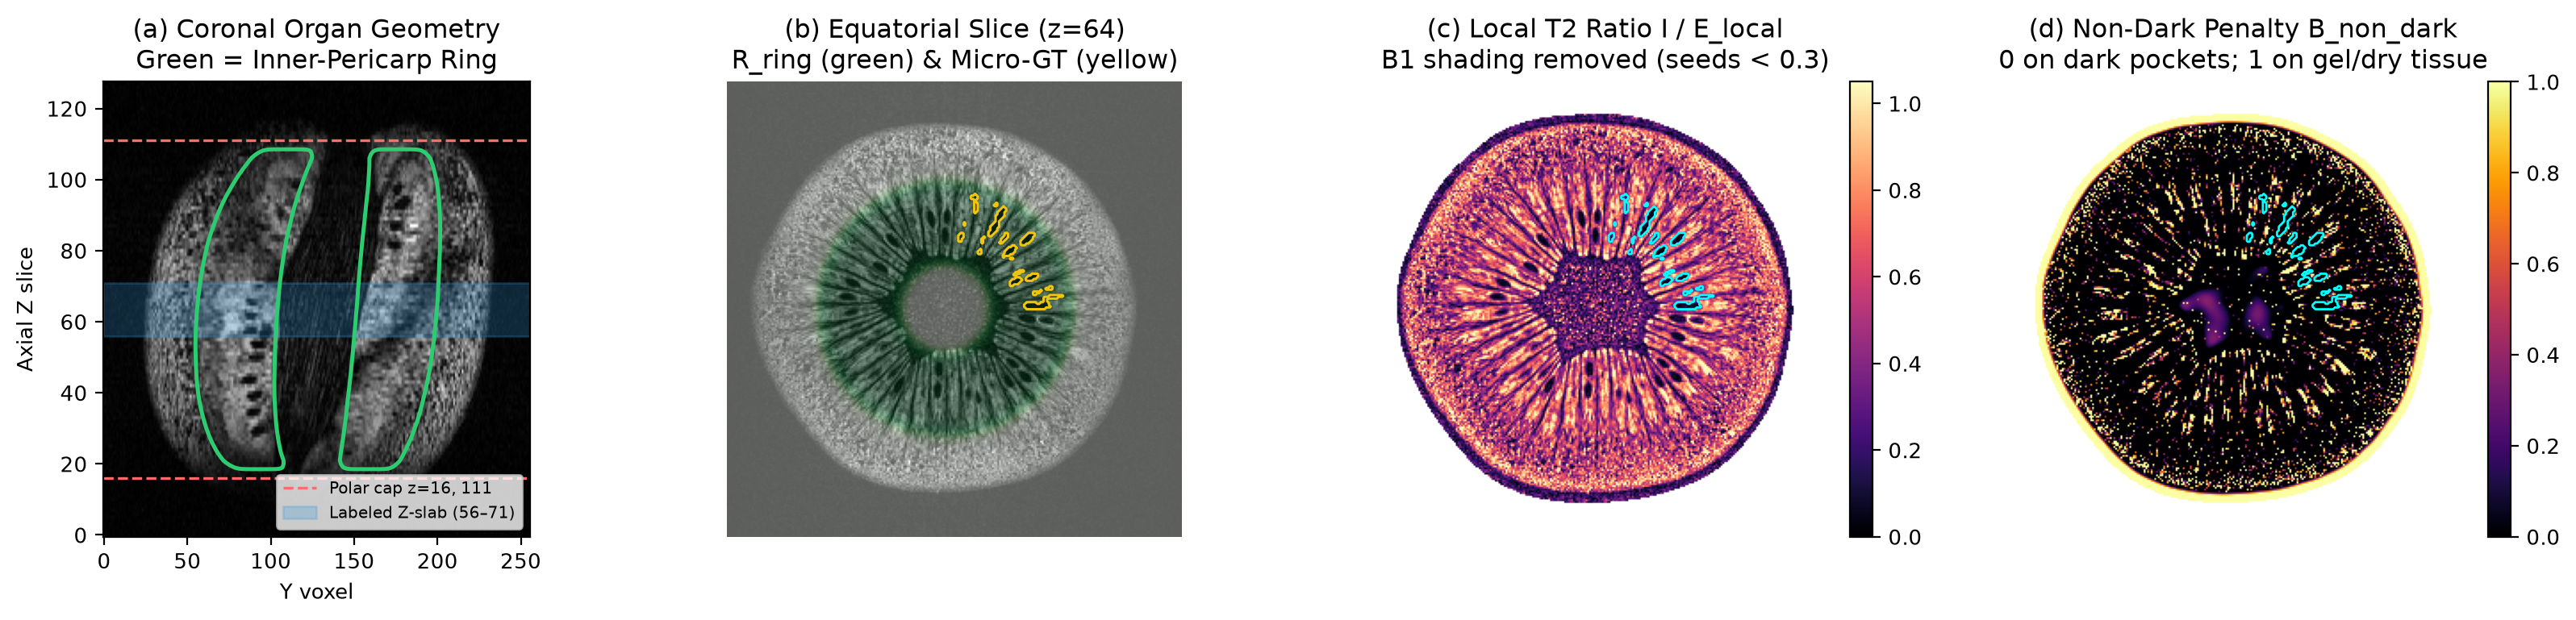
\includegraphics[width=\textwidth]{../figures/fig01_organ_geometry_and_priors.png}
    \vspace{-4pt}
    \caption*{\footnotesize\textit{Executed Figure~1 (\texttt{Out [3]}, saved as \texttt{fig01\_organ\_geometry\_and\_priors.png}): Whole-organ coronal geometry with physical aspect ratio ($2.133\times$), equatorial inner-pericarp membership $R_{\text{ring}}$, $B_1$-invariant local $T_2$ ratio $I/E_{\text{local}}$, and smooth non-dark physics penalty $B_{\text{non\_dark}}$.}}
\end{figure}
\begin{figure}[H]
    \centering
    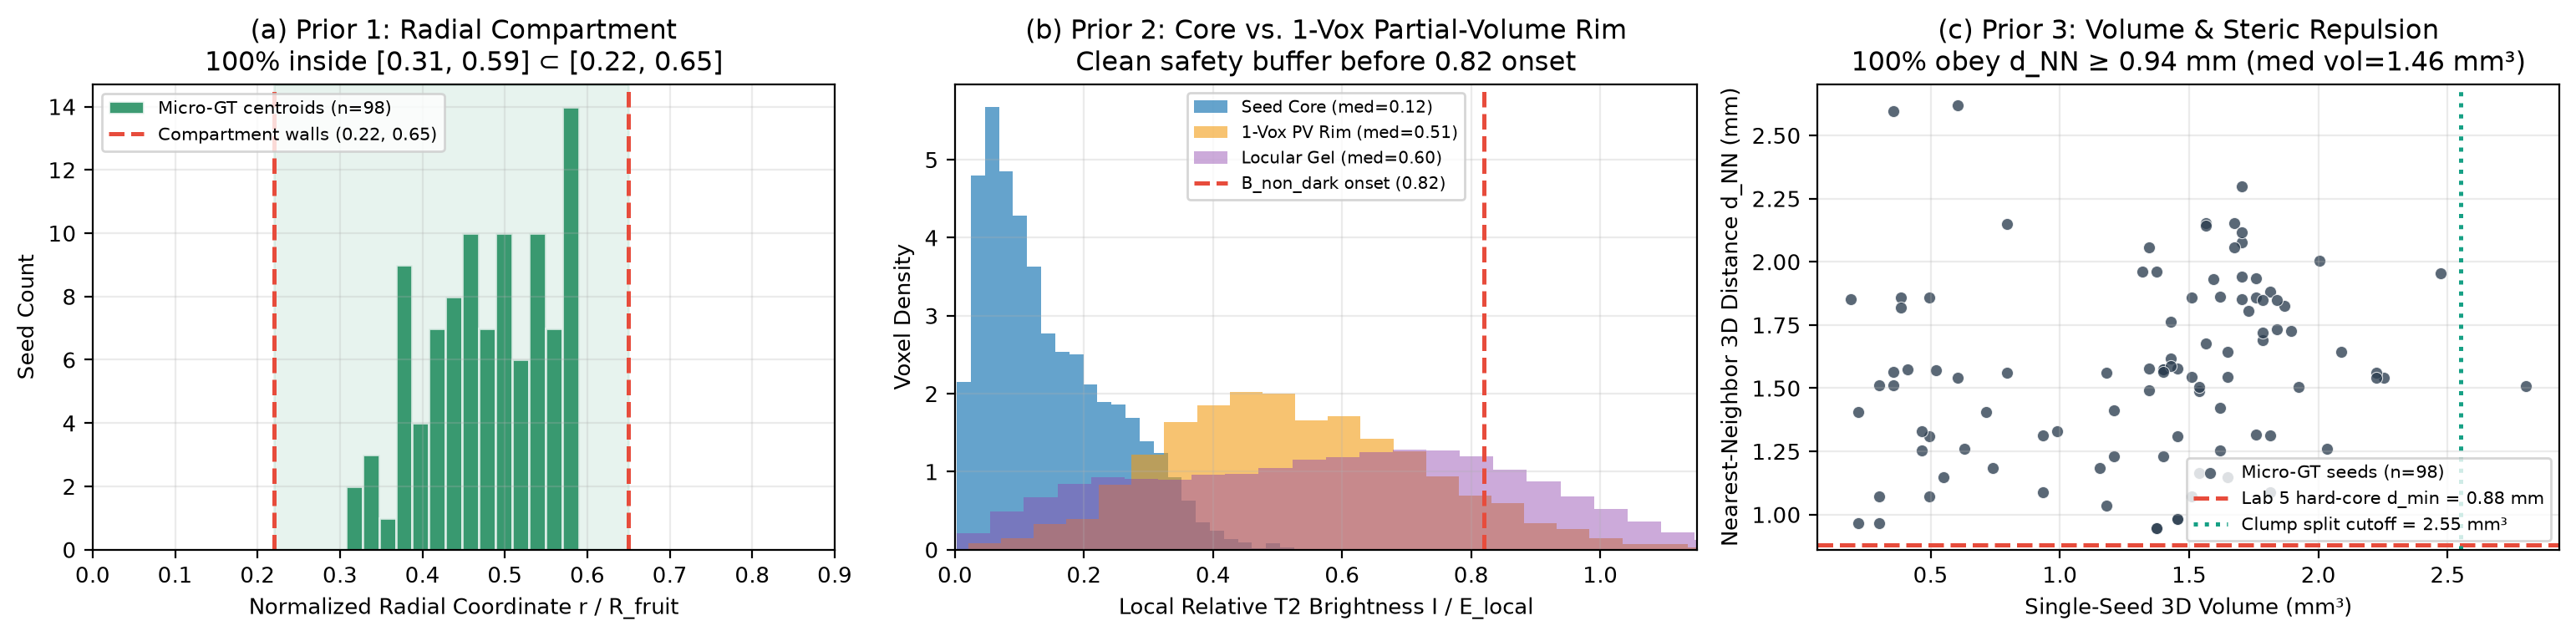
\includegraphics[width=\textwidth]{../figures/fig02_prior_distributions_and_rim.png}
    \vspace{-4pt}
    \caption*{\footnotesize\textit{Executed Figure~2 (\texttt{Out [3]}, saved as \texttt{fig02\_prior\_distributions\_and\_rim.png}): Empirical distributions across all $n = 98$ curated Micro-GT seeds verifying Prior~1 radial containment ($[0.307, 0.590] \subset [0.22, 0.65]$), Prior~2 core vs.\ 1-voxel partial-volume rim vs.\ gel contrast buffer below $0.82$, and Prior~3 Mat\'ern steric floor ($d_{\text{NN}} \ge 0.94\,\text{mm} > 0.88\,\text{mm}$).}}
\end{figure}

\section*{3. Tri-Planar 3D Superimposition Audit \& Silver-Standard Provenance Check}
\addcontentsline{toc}{section}{\texorpdfstring{3. Tri-Planar 3D Superimposition Audit \& Silver-Standard Provenance Check}{3. Tri-Planar 3D Superimposition Audit and Silver-Standard Provenance Check}}

Before training any model, we explicitly audit \textbf{ground-truth provenance and spatial alignment}:
\begin{itemize}
\item \textbf{\texttt{kiwi\_micro\_gt\_labels.nii.gz}} is a \textbf{semi-automated (``silver-standard'') reference mask} generated by \texttt{scripts/\allowbreak{}curate\_micro\_gt.py} (multi-scale 3D LoG + ellipsoidal \texttt{grey\_closing} + bright-locule envelope + 3D watershed + physical-mm $K$-means splitting) refined across multi-slice visual audits --- \textbf{not} manual voxel-by-voxel expert tracing and \textbf{not} destructive physical ground truth.
\item It is stored on the \textbf{exact same \texttt{256 $\times$ 256 $\times$ 128} voxel lattice} with \textbf{bit-identical \texttt{sform} 4$\times$4 affine} (\texttt{max |$\Delta$ affine| = 0.0}) as the raw 7\,T RARE MRI, so it superimposes directly onto the 3D scan in \textbf{FreeSurfer \texttt{freeview}}, \textbf{3D Slicer}, or \textbf{ITK-SNAP} (\texttt{scripts/\allowbreak{}view\_kiwi\_freeview.sh}).
\item Below we verify the tri-planar superimposition (Axial, Coronal, Sagittal in true physical aspect ratio, plus high-magnification test-wedge crop) showing the \textbf{Train Wedge} (\texttt{59} seeds, green), \textbf{Strictly Held-Out Test Wedge} (\texttt{52} seeds, gold), and the \textbf{\texttt{y = 168} (\texttt{y\_split = 40}) cut plane} (cyan dashed, crossed by \texttt{13} straddling seeds).
\end{itemize}

\begin{guidehdr}
{\small\bfseries\color{kiwigreen!75!black}Conceptual \& Mathematical Guide: NIfTI Affine Bit-Alignment \& Spatial Train/\allowbreak{}Test Split Geometry}
\end{guidehdr}

\subsubsection*{3.1 Homogeneous $4 \times 4$ Affine Verification}
In 3D medical imaging (NIfTI-1 format), a voxel array $\mathbf{I} \in \mathbb{R}^{X \times Y \times Z}$ is linked to physical scanner coordinates $(x_{\text{mm}}, y_{\text{mm}}, z_{\text{mm}})$ via a $4 \times 4$ homogeneous \textbf{affine matrix} $\mathbf{A}$:
\[
\begin{bmatrix} x_{\text{mm}} \\ y_{\text{mm}} \\ z_{\text{mm}} \\ 1 \end{bmatrix} = \mathbf{A} \begin{bmatrix} i \\ j \\ k \\ 1 \end{bmatrix}.
\]
Checking $\max|\mathbf{A}_{\text{MRI}} - \mathbf{A}_{\text{GT}}| = 0.0$ (\texttt{ds.gt\_affine\_max\_diff}) proves that our curated reference mask shares the exact lattice origin, orientation, and anisotropic spacing as the raw 7\,T scan---eliminating resampling or sub-voxel shift errors when overlaid in \texttt{freeview}, \texttt{3D Slicer}, or \texttt{ITK-SNAP}.

\subsubsection*{3.2 Leakage-Free Spatial Partition \& Honest Cut-Plane Accounting}
Inside the equatorial $80 \times 80 \times 16$ ROI ($102{,}400 / 8{,}388{,}608 = 1.22\%$ of the full volume), slicing at $y_{\text{cut}} = y_0 + 40 = 168$ divides the ROI into two voxel-disjoint wedges:
\begin{itemize}
\item \textbf{Train Wedge ($\Omega_L$):} $y \in [128, 168)$, containing $|S_{\text{train}}| = 59$ distinct instance IDs.
\item \textbf{Held-Out Test Wedge ($\Omega_{\text{test}}$):} $y \in [168, 208)$, containing $|S_{\text{test}}| = 52$ distinct instance IDs.
\end{itemize}

By the inclusion--exclusion principle, $|S_{\text{train}} \cap S_{\text{test}}| = |S_{\text{train}}| + |S_{\text{test}}| - |S_{\text{ROI}}| = 59 + 52 - 98 = \mathbf{13}$ seeds straddle the $y = 168$ cut plane, contributing disjoint clipped fragments to each side. Logging this exact count in \texttt{nb01\_prior\_audit.json} ensures full methodological transparency.

\subsubsection*{3.3 What the Code Below Computes (Figure 1b)}
\begin{enumerate}
\item Verifies bit-identical affine alignment, counts straddling seed IDs, and appends provenance metadata to \texttt{nb01\_prior\_audit.json}.
\item Alpha-blends emerald green (Train) and gold (Held-Out Test) masks over normalized MRI intensities across \textbf{(a)} Axial (\texttt{z = 64}), \textbf{(b)} Coronal (\texttt{y = 176}, true physical aspect \texttt{2.133}), \textbf{(c)} Sagittal (\texttt{x = 160}, crossing the \texttt{y = 168} split plane), and \textbf{(d)} a high-magnification test-wedge crop assigning distinct \texttt{tab20} colors to individual \texttt{uint16} seed IDs (\texttt{1..98}).
\end{enumerate}

\begin{codebox}[{In [4] $\cdot$ Python --- Tri-planar 3D Micro-GT superimposition audit \& affine verification}]
\begin{lstlisting}[style=pybmed]
# Figure 1b (Report Figure 2): 4-Panel Tri-Planar 3D Superimposition of Silver Micro-GT on Raw 7T MRI
train_ids = set(int(v) for v in np.unique(ds.train_gt) if v > 0)
test_ids = set(int(v) for v in np.unique(ds.test_gt) if v > 0)
straddle_ids = sorted(train_ids & test_ids)

gt_train_full = np.zeros_like(ds.gt_full, dtype=bool)
gt_test_full = np.zeros_like(ds.gt_full, dtype=bool)
y_cut = ds.ry0 + ds.split_y  # 128 + 40 = 168
gt_train_full[ds.rx0:ds.rx1, ds.ry0:y_cut, ds.rz0:ds.rz1] = ds.train_gt > 0
gt_test_full[ds.rx0:ds.rx1, y_cut:ds.ry1, ds.rz0:ds.rz1] = ds.test_gt > 0

print(f"Affine alignment check (max |MRI - GT affine|): {ds.gt_affine_max_diff:.6f} (BIT-IDENTICAL)")
print(f"ROI bounds: x=[{ds.rx0},{ds.rx1}), y=[{ds.ry0},{ds.ry1}), z=[{ds.rz0},{ds.rz1}) | y_cut={y_cut}")
print(f"Train seeds={len(train_ids)}, Test seeds={len(test_ids)}, Cut-plane straddling seeds={len(straddle_ids)}")

# Append provenance metrics to nb01_prior_audit.json
audit_path = RES_DIR / "nb01_prior_audit.json"
audit_j = json.loads(audit_path.read_text(encoding="utf-8"))
audit_j.update({
    "gt_standard": "semi-automated silver-standard (scripts/curate_micro_gt.py + visual audit)",
    "gt_affine_max_diff": round(float(ds.gt_affine_max_diff), 8),
    "roi_vox_pct_of_volume": round(100.0 * (80 * 80 * 16) / float(np.prod(ds.vol.shape)), 2),
    "n_cut_plane_straddling_seeds": len(straddle_ids),
})
audit_path.write_text(json.dumps(audit_j, indent=2), encoding="utf-8")

def blend_overlay(gray_2d: np.ndarray, m_tr: np.ndarray, m_te: np.ndarray) -> np.ndarray:
    g = np.clip(gray_2d / max(float(np.percentile(gray_2d, 99.5)), 1e-6), 0.0, 1.0)
    rgb = np.stack([g, g, g], axis=-1)
    rgb[m_tr] = 0.42 * rgb[m_tr] + 0.58 * np.array([0.12, 0.88, 0.42])   # Emerald green = Train Wedge
    rgb[m_te] = 0.38 * rgb[m_te] + 0.62 * np.array([1.00, 0.78, 0.08])   # Gold/Amber = Held-Out Test Wedge
    return np.clip(rgb, 0.0, 1.0)

fig, axes = plt.subplots(1, 4, figsize=(17.4, 4.1))
asp_xz = ds.spacing[2] / ds.spacing[0]  # 0.50 / 0.2344 = 2.133 (true physical mm aspect!)

# (a) Axial slice z=64 zoomed cleanly to the equatorial sector
z_ax = 64
ax_rgb = blend_overlay(ds.vol_norm[:, :, z_ax].T, gt_train_full[:, :, z_ax].T, gt_test_full[:, :, z_ax].T)
axes[0].imshow(ax_rgb, origin="lower")
axes[0].plot([ds.rx0, ds.rx1, ds.rx1, ds.rx0, ds.rx0], [ds.ry0, ds.ry0, ds.ry1, ds.ry1, ds.ry0],
             color="#ff5252", lw=1.4, ls="--", label="Micro-GT ROI (80×80)")
axes[0].plot([ds.rx0, ds.rx1], [y_cut, y_cut], color="#00e5ff", lw=1.6, ls="--", label=f"y_split={y_cut} cut")
axes[0].set_xlim(90, 232)
axes[0].set_ylim(90, 232)
axes[0].set_xlabel("X voxel")
axes[0].set_ylabel("Y voxel")
axes[0].set_title(f"(a) Axial Superimposition (z={z_ax})\nGreen=Train(59) | Gold=Test(52)")
axes[0].legend(fontsize=7.0, loc="lower left")

# (b) Coronal slice y=176 (inside Held-Out Test Wedge) in true physical mm aspect
y_cor = 176
cor_rgb = blend_overlay(ds.vol_norm[:, y_cor, :].T, gt_train_full[:, y_cor, :].T, gt_test_full[:, y_cor, :].T)
axes[1].imshow(cor_rgb, origin="lower", aspect=asp_xz)
axes[1].plot([ds.rx0, ds.rx1, ds.rx1, ds.rx0, ds.rx0], [ds.rz0, ds.rz0, ds.rz1, ds.rz1, ds.rz0],
             color="#ff5252", lw=1.3, ls="--")
axes[1].set_xlim(35, 225)
axes[1].set_ylim(18, 110)
axes[1].set_xlabel("X voxel")
axes[1].set_ylabel("Axial Z slice (true mm aspect)")
axes[1].set_title(f"(b) Coronal View (y={y_cor}, Test)\nAnisotropic Δz=0.50 mm (2.13×)")

# (c) Sagittal slice x=160 crossing the y=168 train/test cut plane in true physical mm aspect
x_sag = 160
sag_rgb = blend_overlay(ds.vol_norm[x_sag, :, :].T, gt_train_full[x_sag, :, :].T, gt_test_full[x_sag, :, :].T)
axes[2].imshow(sag_rgb, origin="lower", aspect=asp_xz)
axes[2].plot([ds.ry0, ds.ry1, ds.ry1, ds.ry0, ds.ry0], [ds.rz0, ds.rz0, ds.rz1, ds.rz1, ds.rz0],
             color="#ff5252", lw=1.3, ls="--")
axes[2].plot([y_cut, y_cut], [ds.rz0, ds.rz1], color="#00e5ff", lw=1.6, ls="--")
axes[2].set_xlim(35, 225)
axes[2].set_ylim(18, 110)
axes[2].set_xlabel("Y voxel")
axes[2].set_ylabel("Axial Z slice (true mm aspect)")
axes[2].set_title(f"(c) Sagittal View (x={x_sag})\nTrain vs. Test across y={y_cut} plane")

# (d) High-magnification voxel-level overlay inside Held-Out Test Wedge (z=64)
zx0, zx1, zy0, zy1 = 132, 186, 166, 206
zoom_gray = ds.vol_norm[zx0:zx1, zy0:zy1, z_ax].T
zoom_lbl = ds.gt_full[zx0:zx1, zy0:zy1, z_ax].T
axes[3].imshow(zoom_gray, cmap="gray", origin="lower", vmin=0.0, vmax=1.0)
# Distinct per-instance color overlay (semi-transparent) + crisp contours
uniq_z = [int(v) for v in np.unique(zoom_lbl) if v > 0]
cmap_inst = plt.get_cmap("tab20")
rgba_z = np.zeros((*zoom_lbl.shape, 4), dtype=np.float32)
for idx_u, uid in enumerate(uniq_z):
    r_c, g_c, b_c, _ = cmap_inst(idx_u % 20)
    rgba_z[zoom_lbl == uid] = (r_c, g_c, b_c, 0.52)
axes[3].imshow(rgba_z, origin="lower")
axes[3].contour(zoom_lbl > 0, levels=[0.5], colors=["#ffeb3b"], linewidths=0.9)
axes[3].set_title(f"(d) High-Mag Test Overlay (z={z_ax})\nBit-aligned affine (Δ=0.0); 1..98 IDs")
axes[3].axis("off")

plt.tight_layout()
fig.savefig(FIG_DIR / "fig01b_triplanar_gt_superimposition.png", bbox_inches="tight", dpi=150)
plt.show()
\end{lstlisting}
\end{codebox}
\begin{outbox}[{Out [4] $\cdot$ stdout}]
\begin{lstlisting}[style=outbmed]
Affine alignment check (max |MRI - GT affine|): 0.000000 (BIT-IDENTICAL)
ROI bounds: x=[128,208), y=[128,208), z=[56,72) | y_cut=168
Train seeds=59, Test seeds=52, Cut-plane straddling seeds=13
\end{lstlisting}
\end{outbox}
\begin{figure}[H]
    \centering
    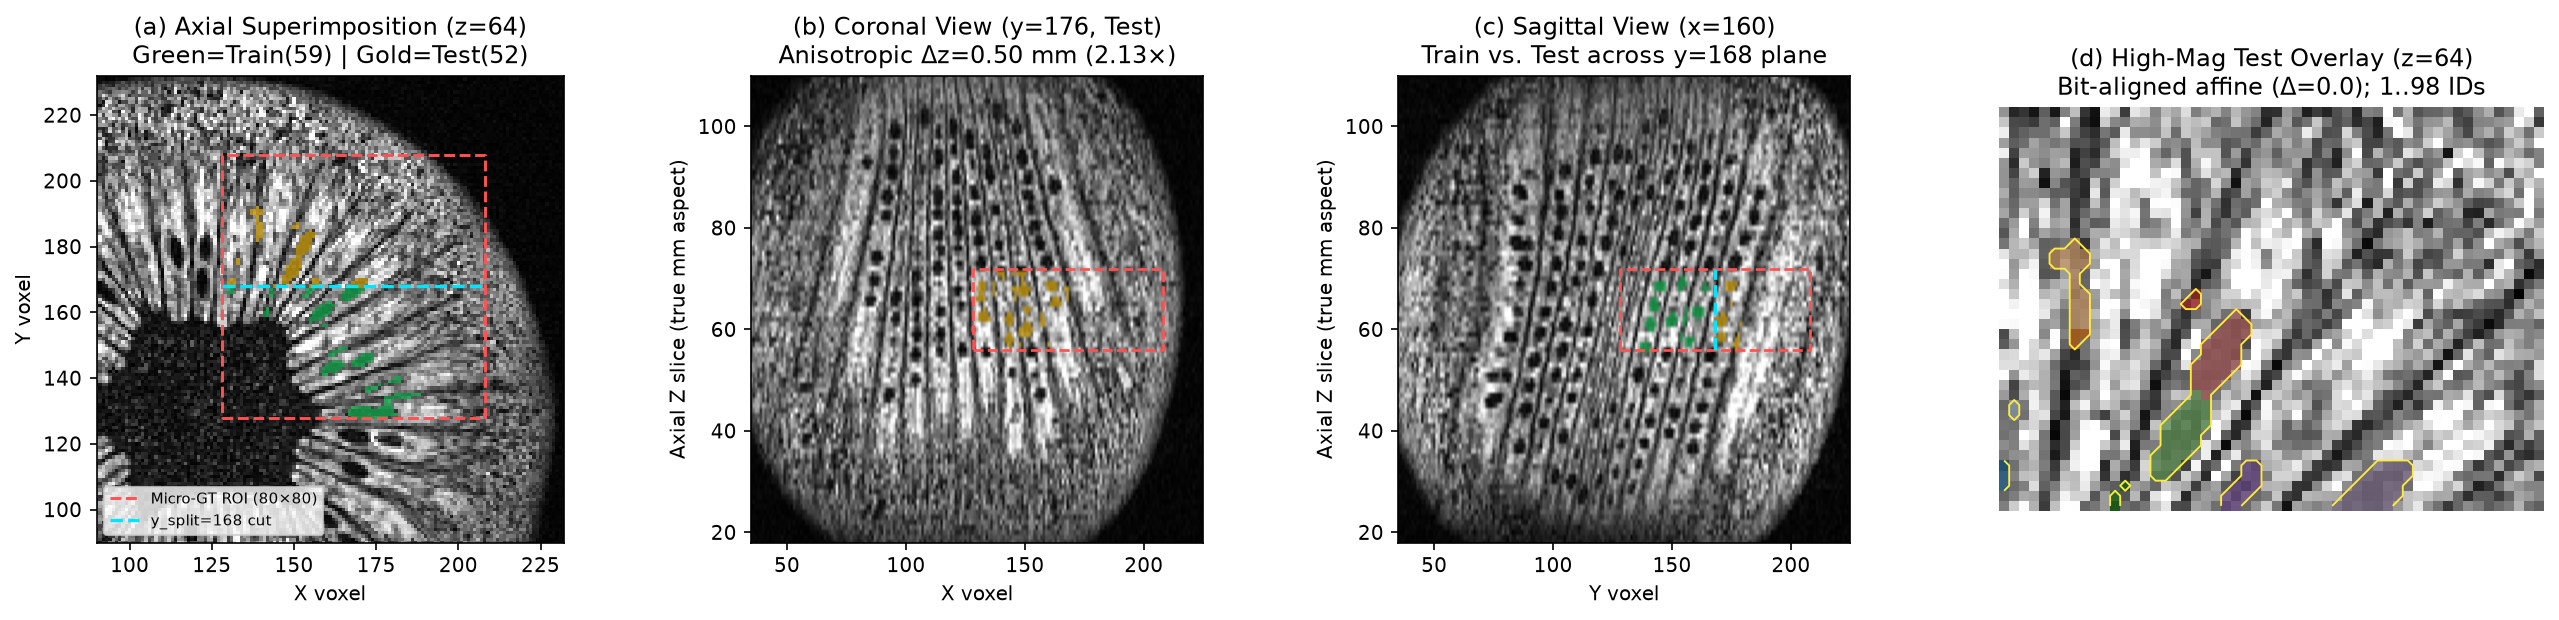
\includegraphics[width=\textwidth]{../figures/fig01b_triplanar_gt_superimposition.png}
    \vspace{-4pt}
    \caption*{\footnotesize\textit{Executed Figure~1b / Report Figure~2 (\texttt{Out [4]}, saved as \texttt{fig01b\_triplanar\_gt\_superimposition.png}): Tri-planar 3D superimposition of the bit-aligned silver-standard Micro-GT ($\max|\Delta\mathbf{A}| = 0.0$) on the raw 7\,T RARE MRI across Axial, Coronal, Sagittal ($2.133\times$ aspect), and high-magnification test-wedge views showing Train (59 seeds, green), Held-Out Test (52 seeds, gold), and the $y = 168$ split plane.}}
\end{figure}

\section*{4. Manual Ground-Truth Refinement: Workflow Impact \& \texttt{freeview} /\allowbreak{} \texttt{ITK-SNAP} Procedures}
\addcontentsline{toc}{section}{\texorpdfstring{4. Manual Ground-Truth Refinement: Workflow Impact \& \texttt{freeview} /\allowbreak{} \texttt{ITK-SNAP} Procedures}{4. Manual Ground-Truth Refinement: Workflow Impact and freeview / ITK-SNAP Procedures}}

\subsection*{4.1 What Happens to the Workflow, Predictions, and Evaluations If You Manually Adjust the GT?}

Because \texttt{kiwi\_ns\_lib.py} reads whatever positive integer instance IDs exist in the GT mask dynamically (handling arbitrary non-contiguous \texttt{uint16} IDs via \texttt{np.unique} and \texttt{measure.regionprops}), manual GT refinement operates in two distinct scientific regimes:

\subsubsection*{A. Evaluation-Only Adjustment (Frozen Model, Updated Held-Out Test Wedge \texttt{y >= 168})}
\begin{itemize}
\item \textbf{Model predictions do not change}, including whole-organ OOD safety (\texttt{0} polar FPs, \texttt{-99.92\%} OOD voxels) and the learned \texttt{Organ-GPS} spatial prior \texttt{z\_GPS}.
\item \textbf{Reported metrics shift diagnostically} to reveal reference-standard sensitivity:
\begin{itemize}
\item \textbf{Adding missed faint/\allowbreak{}small seeds} or \textbf{deleting false-positive septa} directly shifts \texttt{TP}, \texttt{FP}, \texttt{FN}, \texttt{Recall}, and \texttt{RQ} (testing whether the model's test \texttt{FP}s are actually real seeds missed by the silver standard).
\item \textbf{Tightening or expanding 1-voxel seed boundaries} shifts \textbf{Semantic Dice} and \textbf{Segmentation Quality (\texttt{SQ})} substantially---because a 40--60-voxel 3D seed changes 3D IoU by \texttt{\textasciitilde{}15--25\%} from a single-voxel rim shift.
\item \textbf{Splitting a fused GT pair} (into two distinct integer IDs) or \textbf{merging an over-split seed} directly changes \texttt{Merges}/\allowbreak{}\texttt{Splits} and \texttt{PQ}.
\item \textbf{Ratio-calibrated whole-fruit count} ($\hat{N}_{\text{cal}} = N_{\text{wf}} \cdot N_{\text{GT,ROI}} / N_{\text{pred,ROI}}$) scales proportionally with the revised ROI seed count.
\end{itemize}
\end{itemize}

\subsubsection*{B. Full Pipeline Re-Run (Manually Adjusted Train Wedge \texttt{y < 168} + Test Wedge \texttt{y >= 168})}
Pass your manually edited NIfTI path via \texttt{ds = kns.load\_kiwi\_dataset(gt\_nii\_override="MyStuff/\allowbreak{}kiwi-gt/\allowbreak{}kiwi\_gt\_manual\_v1.nii.gz")} across Notebooks \texttt{01}--\texttt{05} without touching the shared silver standard in \texttt{data/\allowbreak{}}:
\begin{enumerate}
\item \textbf{Prior Audit (\texttt{NB 01}) breaks silver-standard circularity:} Recomputing radial bounds \texttt{r/\allowbreak{}R}, core vs. 1-voxel PV rim \texttt{I/\allowbreak{}E\_local}, single-seed volume IQR, and \texttt{d\_NN} on human-curated labels immediately verifies whether Priors 1--3 (\texttt{[0.22, 0.65]}, \texttt{0.82} onset, \texttt{d\_min = 0.88 mm}, \texttt{V\_split = 2.55 mm\textsuperscript{3}}) match human judgment or need updating \textit{before} training.
\item \textbf{Supervised targets rebuild automatically:} \texttt{build\_distance\_targets()} recomputes both the binary foreground mask and per-instance normalized 3D Euclidean Distance Transform (\texttt{y\_d}) for every edited, added, or split seed ID in \texttt{train\_gt}.
\item \textbf{Threshold calibration adapts automatically:} \texttt{calibrate\_threshold\_on\_train()} automatically re-locks $\tau_{\text{fg}}^*$ to match your annotation style (higher $\tau_{\text{fg}}^*$ for tight dark cores; lower $\tau_{\text{fg}}^*$ if dimmer PV rims are included).
\item \textbf{Unsupervised SSL \& LTN unlabeled blocks ($\Omega_U$) remain unchanged}, while the trade-off between human supervised labels ($\mathcal{L}_{\text{sup}}$) and biophysical domain rules ($\mathcal{L}_{\text{anat}} + \mathcal{L}_{\text{phys}}$) adapts cleanly.
\end{enumerate}

\vspace{0.25em}\noindent\textcolor{uibblue!25}{\rule{\linewidth}{0.4pt}}\vspace{0.25em}

\subsection*{4.2 How to Manually Adjust the GT Safely (Golden Rule + Step-by-Step Procedures)}

\begin{clinbox}[Golden Rule for 3D Instance Masks (\texttt{uint16})]
\texttt{kiwi\_micro\_gt\_labels.nii.gz} stores \textbf{per-seed integer IDs} (\texttt{0 = background}, \texttt{1..98 = individual seeds}) inside \texttt{x $\in$ [128, 207]}, \texttt{y $\in$ [128, 207]}, \texttt{z $\in$ [56, 71]} (\texttt{y\_split = 168}).
\begin{itemize}
\item To \textbf{refine an existing seed}, paint with \textbf{its exact existing integer ID} (e.g. \texttt{42}) or erase to \texttt{0}.
\item To \textbf{add a new seed} or \textbf{split a fused twin}, paint with a \textbf{brand-new unused integer ID} (\texttt{99}, \texttt{100}, \texttt{101}, \ldots{}) --- never reuse a touching neighbor's ID, or the two blobs will merge into one instance.
\item \textbf{Always edit a working copy in git-ignored \texttt{MyStuff/\allowbreak{}kiwi-gt/\allowbreak{}}} so the shared silver standard stays untouched and Notebook \texttt{03b} can auto-discover it for inter-rater Dice /\allowbreak{} Cohen's $\kappa$ /\allowbreak{} \texttt{STAPLE} consensus!
\end{itemize}
\end{clinbox}

Create a personal working copy from the repository root:
\begin{lstlisting}[style=bashbmed]
mkdir -p MyStuff/kiwi-gt
cp Lab4-Comp-Imag/Kiwi-challenge/data/kiwi_micro_gt_labels.nii.gz \
   MyStuff/kiwi-gt/kiwi_gt_manual_v1.nii.gz
\end{lstlisting}

\subsubsection*{Procedure A: Manual Voxel Editing in FreeSurfer 8.2.0 \texttt{freeview} (macOS)}
\begin{enumerate}
\item \textbf{Launch \texttt{freeview} on your working copy} using our launcher script (automatically attaches our custom high-contrast \texttt{kiwi\_seeds\_ColorLUT.txt} supporting vivid distinct colors for IDs \texttt{1..2000}):
\begin{lstlisting}[style=bashbmed]
./Lab4-Comp-Imag/Kiwi-challenge/scripts/view_kiwi_freeview.sh --gt MyStuff/kiwi-gt/kiwi_gt_manual_v1.nii.gz
\end{lstlisting}
\item \textbf{Enter Voxel Edit mode:} Select \texttt{Custom\_Manual\_GT} in the left \textit{Volumes} list $\to$ click \textbf{Voxel Edit} (pencil icon, or \textit{Tools $\to$ Voxel Edit} /\allowbreak{} \texttt{Cmd+E}). Set \textbf{Brush Size = \texttt{1}} (or \texttt{2}) in \textbf{2D} brush mode (avoiding accidental spillover across the \texttt{0.50 mm} thick $z$-slices).
\item \textbf{Edit seed instances:}
\begin{itemize}
\item Hover over any seed to read its integer ID (\texttt{1..98}) in the bottom \textit{Cursor} panel.
\item \textbf{Expand/\allowbreak{}shrink an existing seed:} Enter its exact ID in \textit{Brush Value}; \textbf{Left-drag} to paint, \textbf{Shift + Left-drag} to erase back to \texttt{0}.
\item \textbf{Delete a false-positive blob:} Select the \textbf{Fill} tool and \textbf{Shift + Click} the blob across its slices.
\item \textbf{Add a new seed or split a fused twin:} Enter an unused ID (\texttt{99}, \texttt{100}, \ldots{}) in \textit{Brush Value} and paint across its 2--4 axial slices while checking Coronal/\allowbreak{}Sagittal compactness.
\item Toggle overlay visibility anytime with \textbf{\texttt{Alt+V}}; undo/\allowbreak{}redo with \textbf{\texttt{Cmd+Z}} /\allowbreak{} \textbf{\texttt{Cmd+Shift+Z}}.
\end{itemize}
\item \textbf{Save:} With \texttt{Custom\_Manual\_GT} selected, press \textbf{\texttt{Cmd+S}} (\textit{File $\to$ Save Volume}).
\end{enumerate}

\subsubsection*{Procedure B: Manual Editing in \texttt{ITK-SNAP} (Especially Fast for 3D Clump Splitting)}
\begin{enumerate}
\item \textbf{Open images:} \textit{File $\to$ Open Main Image} (\texttt{data/\allowbreak{}kiwi\_20050217191129\_131073\_RARE\_high\_res\_axial.nii.gz}) $\to$ \textit{Segmentation $\to$ Open Segmentation} (\texttt{MyStuff/\allowbreak{}kiwi-gt/\allowbreak{}kiwi\_gt\_manual\_v1.nii.gz}) $\to$ jump cursor to \texttt{(168, 168, 64)} and click \textbf{Update} in the 3D pane.
\item \textbf{Edit instances:} Press \textbf{\texttt{3}} (Paintbrush) or \textbf{\texttt{2}} (Polygon); press \textbf{\texttt{S}} to toggle visibility. Add unused IDs (\texttt{99}, \texttt{100}, \ldots{}) via \textit{Segmentation $\to$ Label Editor}. Set \textit{Paint over = \texttt{Clear Label}} when refining near neighbors, or \texttt{All Labels} when carving out half of a fused pair with a new ID. Use the \textbf{3D Scalpel tool (\texttt{6})} in the 3D window to slice a fused twin clump along a single plane and reassign one half to a new ID in one step.
\item \textbf{Save:} \textit{Segmentation $\to$ Save Segmentation Image} $\to$ \texttt{MyStuff/\allowbreak{}kiwi-gt/\allowbreak{}kiwi\_gt\_manual\_v1.nii.gz}.
\end{enumerate}

\subsubsection*{Benchmarking /\allowbreak{} Retraining Against Your Edited GT in Notebooks \texttt{01}--\texttt{05}}
\begin{lstlisting}[style=pybmed]
ds = kns.load_kiwi_dataset(gt_nii_override="MyStuff/kiwi-gt/kiwi_gt_manual_v1.nii.gz")
\end{lstlisting}

\end{document}
